\begin{block}{Maximizing Quantum Boost} 
    Experiments show that the D-Wave solver makes marginal use of the QPU: average contribution of \textbf{0.08\%}. 
    For greater performance, we run the problem directly on the QPU: bypass the opaque workflow D-Wave proprietary technology hybrid solvers.
   
    We transform the learning of an SVM into a problem that is solvable directly by the QPU. Among the series of required steps, the only one impacting performance is the calculation of a minor embedding\cite{MEdwave}.
   
    \begin{figure}[h!]
        \centering
        \begin{minipage}{0.55\textwidth}
        \begin{alertblock}{QPU Bottleneck}
            Empirically, we identify a sweet spot for problems with 32 variables.
                        
            Beyond this size, the time required to find the minor graph can become dominant compared to the time needed to solve the problem.

            Additionally, the number of qubits required to represent the problem graph becomes incompatible with the current QPU sizes (approximately 5600 qubits).
        \end{alertblock}
        \end{minipage}%
        \hfill
        \begin{minipage}{0.4\textwidth}
            \centering
            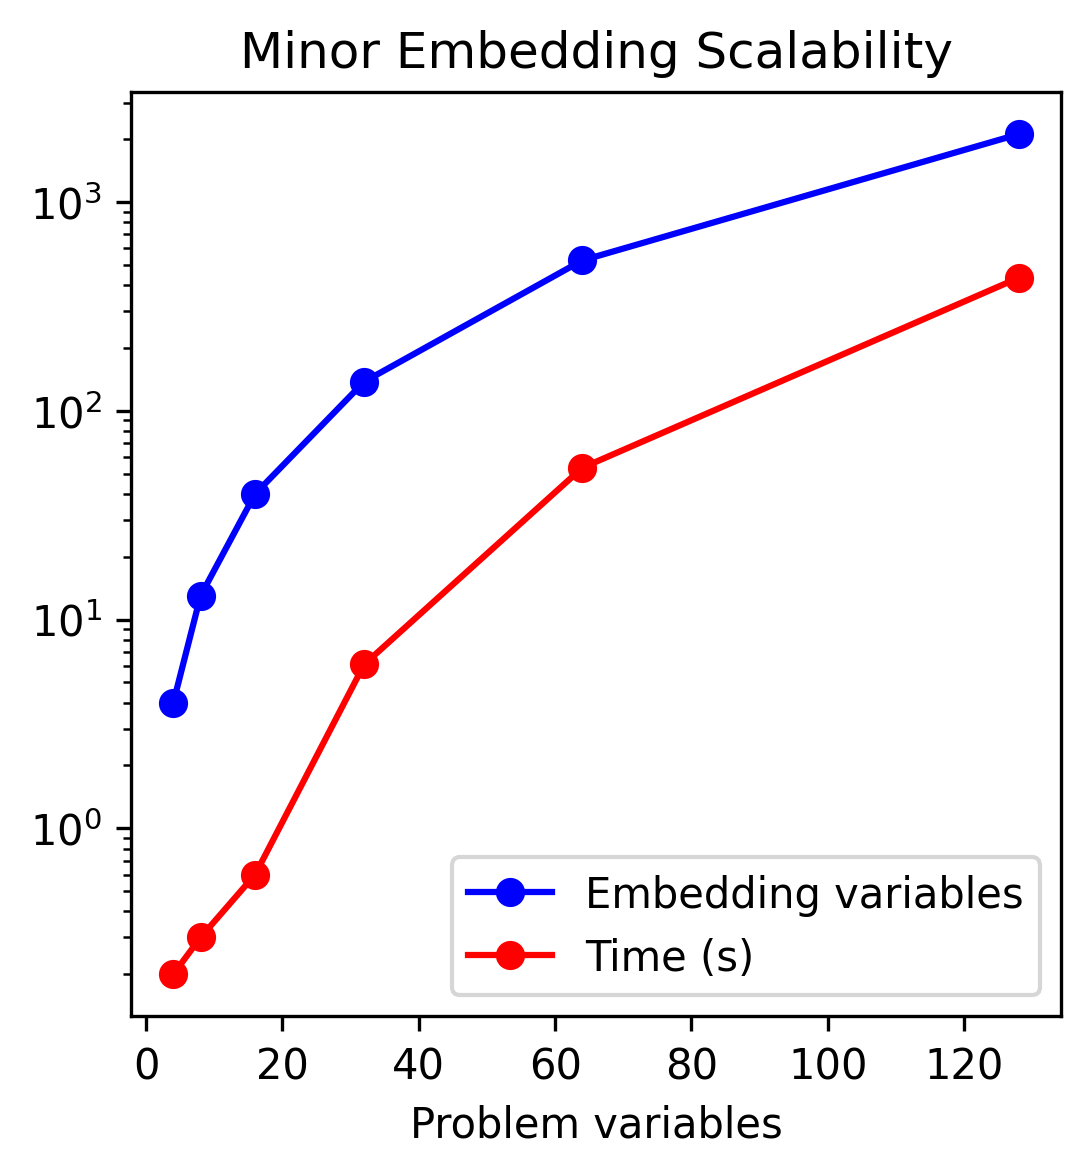
\includegraphics[height=0.14\textheight]{logos/embedding_search_time.png}
        \end{minipage}
    \end{figure}
\end{block}